\documentclass{beamer}
%%%%%%%%%%%%%%%%%%%%%%%%%%%%%%%%%%%%%%%%%%%%%%%%%%%%%%%%%%%%%%%%%%%%%%%%%%%%
\usepackage{bm}
\usepackage{amsmath}
\usepackage{amssymb}
%\usepackage{microtype}
\usepackage{booktabs} % \toprule, \midrule, \bottomrule
%%% INCLUDE FILE FOR DEFINITIONS
%%% These may require various packages.

% Shortcuts in regular text
\newcommand{\degs}{\ensuremath{^\circ}}
\newcommand{\EE}[1]{\ensuremath{\times 10^{#1}}}
\newcommand{\ttimes}{\ensuremath{{}\times{}}}
\newcommand{\cclicense}{%
  \smash{\raisebox{-0.45ex}{%
  \setlength{\unitlength}{1em}%
  \begin{picture}(1,1)%
    \put(0.5,0.5){\circle{1}}
    \put(0.5,0.5){\hbox to 0pt{\hss\raisebox{-.45ex}{\tiny\textsf{CC}}\hss}}
  \end{picture}%
  }}%
  \hskip -1em%
  \href{http://creativecommons.org/licenses/by-nc-sa/3.0/}%
  {\ \hskip 1em \textsf{BY-NC-SA}}%
}

%\newcommand{\horizsep}{{\par\noindent\centering\rule[.25ex]{.75\columnwidth}{2pt}\par}}
\newcommand{\horizsep}{\vspace{\baselineskip}\noindent\hspace{\stretch{1}}$
\ast\qquad \ast\qquad \ast\qquad
$ \hspace{\stretch{1}} \vspace{\baselineskip}}
\newcommand{\pytrt}{\textsf{PyTRT}}

% Research
\newcommand{\lop}[1]{\mathcal{L}\!\left[#1\right]}
\newcommand{\lopinv}[2]{\mathcal{I}_{#1}\!\left[#2\right]}
\newcommand{\Dtens}{\mat{D}}
\newcommand{\Etens}{\mat{E}}
\newcommand{\Identitytens}{\mat{I}}
\newcommand{\APone}{AP$_1$}
\newcommand{\Pone}{P$_1$}
\newcommand{\SN}{S$_N$}%{S$_\text{N}$}%{$S_N$}%
\newcommand{\PN}{P$_N$}%{P$_\text{N}$}%{$P_N$}%
\newcommand{\CN}{Crank--Nicolson} %Yes, it's Nic not Nich
\newcommand{\Eddington}{\mathcal{E}} %whatever symbol I decided for Eddington
\newcommand{\RadEn}{E} %whatever symbol I decide for radiation energy
\newcommand{\Sigmatr}{\Sigma_{\mathit{tr}}}

% Program names
\newcommand{\cpp}{\textsf{C\raisebox{0.2ex}{++}}}

% General math shortcuts
\newcommand{\ud}{\mathop{}\!\mathrm{d}}
\newcommand{\pder}[2]{\frac{\partial #1}{\partial #2}}
\newcommand{\oder}[2]{\frac{\mathrm{d} #1}{\mathrm{d} #2}}
\newcommand{\tpder}[2]{{\partial #1}/{\partial #2}} %inlined
\newcommand{\toder}[2]{{\mathrm{d} #1}/{\mathrm{d} #2}} %inlined
\newcommand{\lra}{ \quad \Longrightarrow \quad }
\newcommand{\eexp}{\mathop{}\!\mathrm{e}} % upright ``e'' for exponent
\newcommand{\expp}[1]{\exp\!\left( {#1} \right)} % exp with parentheses
\newcommand{\qeq}{\stackrel{\mathrm{?}}{=}}

% Probability
\newcommand{\expectation}[1]{\mathop{}\!\mathrm{E}\!\left[ #1 \right]}
\DeclareMathOperator{\Var}{Var} % variance

% Asymptotic analysis
\DeclareMathOperator{\Ei}{Ei} % Exponential function
\newcommand{\lapl}[1]{\mathcal{L}[{#1}]} %laplace

%change the Re and Im operators from fancy curly letters
\DeclareMathOperator{\MathOpRe}{Re}
\renewcommand{\Re}{\MathOpRe}
\DeclareMathOperator{\MathOpIm}{Im}
\renewcommand{\Im}{\MathOpIm}

%imaginary ``i'' , upright 'i' or \imath
\newcommand{\iimag}{\mathrm{i}}

% Finite differences
\newcommand{\hot}{\text{h.o.t.}}
\newcommand{\inv}{^{-1}}

% Numerical Linear Algebra
\newcommand{\conj}{^{\ast}} % complex conjugate (transpose)
\newcommand{\norm}[1]{\left\| #1 \right\|} % double pipe
\newcommand{\abs}[1]{\left| #1 \right|} % single pipe
\newcommand{\eps}{\varepsilon}
\DeclareMathOperator{\fl}{fl}

\DeclareMathOperator{\acosh}{arccosh} 

% Define a command to write a nice-looking element, e.g. 4,2 He
\newcommand{\elem}[3]{\ensuremath{{}^{{#1}}_{{#2}}\mathrm{{#3}}}}

% Vector definitions
\newcommand{\mat}[1]{\mathbf{#1}} %matrix is bold upright
\renewcommand{\vec}[1]{\bm{#1}} %vector is bold italic
\newcommand{\op}[1]{\mathsf{#1}} % ``operator'' is sans serif

\newcommand{\vd}{\bm{\cdot}} % slightly bold vector dot
\newcommand{\del}{\vec{\nabla}} % gradient (Del) is bold
\newcommand{\grad}{\vec{\nabla}} % gradient

%\newcommand{\abr}[1]{\langle {#1} \rangle}
\newcommand{\abr}[1]{\left\langle {#1} \right\rangle} % angle brackets for avg.

%% topbox is useful in extended definitions of math terms inside an align
\newcommand{\topbox}[2][0.6]{\parbox[t]{#1\columnwidth}{\raggedright{}#2}}

% commands to make text in math mode appear as zero-width (better-looking
% integrals/sums, e.g.)
% from mathmode.pdf page 74, or Alexander R. Perlis ``A complement to \smash,
% \llap, and \rlap''

\def\mathllap{\mathpalette\mathllapinternal}
	\def\mathllapinternal#1#2{%
	\llap{$\mathsurround=0pt#1{#2}$}%
}
\def\clap#1{\hbox to 0pt{\hss#1\hss}}%
\def\mathclap{\mathpalette\mathclapinternal}%
\def\mathclapinternal#1#2{%
	\clap{$\mathsurround=0pt#1{#2}$}%
}
\def\mathrlap{\mathpalette\mathrlapinternal}%
\def\mathrlapinternal#1#2{%
	\rlap{$\mathsurround=0pt#1{#2}$}%
}

\setSRJthesisfigurepaths

\definecolor{lightgray}{gray}{0.85}
\newcommand{\epsiloncolor}[1]{\textcolor{blue}{#1}}

%%%%%%%%%%%%%%%%%%%%%%%%%%%%%%%%%%%%%%%%%%%%%%%%%%%%%%%%%%%%%%%%%%%%%%%%%%%%

\usetheme{AnnArbor}
\usecolortheme{seahorse}
\usecolortheme{orchid}
\usefonttheme[onlymath]{serif}
\setbeamercolor*{frametitle}{use=structure,bg=structure.fg!20!white}
\setbeamercolor*{frametitle right}{use=structure,bg=structure.fg!20!white}
\setbeamertemplate{navigation symbols}{\insertframenavigationsymbol}
\setbeamertemplate{caption}[numbered]

\title[Thesis Prospectus]%
{A Physics-Based Anisotropic Diffusion Method for Thermal Radiative
Transfer}
%\subtitle{}

\author[SRJ]{Seth~R.~Johnson}

\institute[UMich]{
University of Michigan, Ann Arbor
}
\date[11/3/2010]{November 3, 2010}

\AtBeginSection[]
{
\begin{frame}
  \frametitle{Outline}
  \tableofcontents[currentsection]
\end{frame}
}

\hypersetup{colorlinks=true,linkcolor=black}

% only show section headings in table of contents
\setcounter{tocdepth}{1}

%use symbols for footnote
\renewcommand{\thefootnote}{\fnsymbol{footnote}}

\begin{document}
%%%%%%%%%%%%%%%%%%%%%%%%%%%%%%%%%%%%%%%%%%%%%%%%%%%%%%%%%%%%%%%%%%%%%%%%%%%%

\begin{frame}
\titlepage
\begin{center}
  
\includegraphics[width=0.2\textwidth]{umlogo}
\end{center}
\end{frame}

%%%%%%%%%%%%%%%%%%%%%%%%%%%%%%%%%%%%%%%%%%%%%%%%%%%%%%%%%%%%%%%%%%%%%%%%%%%%
\section{Introduction}
%%%%%%%%%%%%%%%%%%%%%%%%%%%%%%%%%%%%%%%%
\begin{frame}
  \frametitle{Thermal radiative transfer}
  \begin{itemize}
    \item TRT is the dominant heat transfer process in very hot materials
    \item Photons are emitted by black body emission ($\propto T^4$)
    \item Cold material heats up and becomes relatively transparent (
      $\sigma\propto T^{-3}$)
  \end{itemize}

  Applications in high energy density physics:
  \begin{itemize}
    \item Stellar astrophysics, \textcolor[gray]{.5}{strategic astrophysics}
    \item Inertial confinement fusion
    \item CRASH (Center for RAdiative Shock Hydrodynamics) program: ``Assessment
          of Predictive Capability''
  \end{itemize}
  Difficulties in solving:
  \begin{itemize}
    \item High dimensionality of solution phase space $(\vec{x}, \vec{\Omega},
      h\nu, t)$
    \item Highly nonlinear coupled partial differential equations for radiation
      field $I(\vec{x}, \vec{\Omega}, h\nu, t)$ and material energy
  \end{itemize}
\end{frame}

%%%%%%%%%%%%%%%%%%%%%%%%%%%%%%%%%%%%%%%%
\begin{frame}
  \frametitle{Gray TRT equations}
  Common approximations for radiation transport methods development:
  \begin{itemize}
    \item work in a fixed medium, disregarding material advection;
    \item assume local thermodynamic equilibrium (LTE), which uses a single
      material temperature;
    \item neglect thermal conduction in material;
    \item average over all photon energies $h\nu$ (gray).
  \end{itemize}
\begin{subequations} \label{eqs:fullGrayTRT}
  Radiation transfer equation, intensity $I(\vec{x}, \vec{\Omega}, t)$:
\begin{equation} \label{eq:fullGrayTransport}
  \frac{1}{c} \pder{I}{t}
  + \vec{\Omega} \vd \del I +
 \sigma I
  = \frac{\sigma c aT^4}{4\pi} 
  + \frac{c Q}{4\pi}
\end{equation}
  Material energy balance equation:
\begin{equation} \label{eq:fullGrayMaterial}
  \frac{1}{c_v}\pder{T}{t} = \sigma \int_{4\pi}  I \ud \Omega - \sigma c aT^4
\end{equation}
\end{subequations}
\end{frame}
%%%%%%%%%%%%%%%%%%%%%%%%%%%%%%%%%%%%%%%%
\begin{frame}
  \frametitle{Motivation}
\begin{center}
  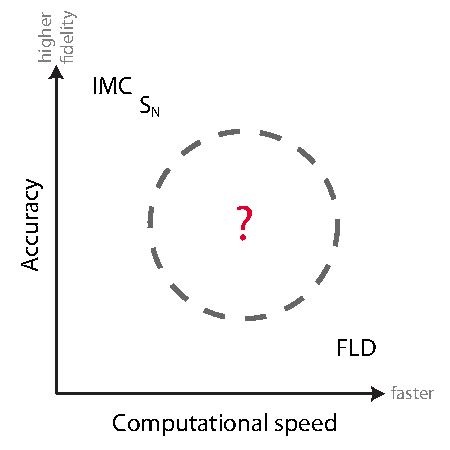
\includegraphics[width=3in]{fidelity}
\end{center}
% also, storage requirements
\end{frame}

%%%%%%%%%%%%%%%%%%%%%%%%%%%%%%%%%%%%%%%%
\begin{frame}
  \frametitle{Anisotropic diffusion work}
  Previous work:
  \begin{itemize}
    \item Steady-state VHTR-like problem with analytically calculated
      coefficients \cite{Lar2009c}
    \item Non-local tensor diffusion \cite{Mor2007} for steady-state
      radiative transfer, no further development or
      analysis in literature
  \end{itemize}
  Current work:
  \begin{itemize}
    \item Time-dependent anisotropic diffusion for thermal radiative transfer!
  \end{itemize}
\end{frame}
%%%%%%%%%%%%%%%%%%%%%%%%%%%%%%%%%%%%%%%%%%%%%%%%%%%%%%%%%%%%%%%%%%%%%%%%%%%%
\section{Theory}
%%%%%%%%%%%%%%%%%%%%%%%%%%%%%%%%%%%%%%%%
\begin{frame}
  \frametitle{Summary in advance}
  \begin{enumerate}
    \item Make assumptions about weakness of derivatives and moments of
      intensity $I(\vec{x}, \vec{\Omega}, t)$.
    \item Convert integrodifferential transport equation to integral transport
      equation along characteristic rays.
    \item Substitute the left hand side of the particle conservation equation
      (zeroth moment of Boltzmann equation) into the integral equation
    \item Apply Taylor series to non-local $\phi$ to get an approximate
      expression for $I(\vec{x}, \vec{\Omega}, t)$ as a function of
      $\phi(\vec{x}, t)$ and other problem-dependent quantities.
      Discard $O(\epsilon^2)$ and higher terms.
    \item Take first moment of this approximate $I$ to get
      $\vec{F}(\vec{x}, t)$.
    \item Apply semi-implicit approximation to TRT equations.
  \end{enumerate}
\end{frame}

\subsection{Anisotropic diffusion derivation}
%%%%%%%%%%%%%%%%%%%%%%%%%%%%%%%%%%%%%%%%
\begin{frame}
  Gray Boltzmann transport equation:
  \begin{multline} \label{eq:fullGrayTransport2}
  \frac{1}{c} \pder{I}{t}(\vec{x}, \vec{\Omega}, t)
  + \vec{\Omega} \vd \del I(\vec{x}, \vec{\Omega}, t) +
 \sigma(\vec{x}, T) I(\vec{x}, \vec{\Omega}, t)
  \\= \frac{\sigma(\vec{x}, T) a c [T(\vec{x},t)]^4}{4\pi} 
  + \frac{c Q(\vec{x},t)}{4\pi}
  %\,, \qquad \vec{x} \in V, \ \vec{\Omega} \in 4\pi, \ t >= 0.
  \end{multline}
  Radiation energy conservation by integrating over angles $\int_{4\pi} (\cdot) \ud
  \Omega$:
  \begin{equation} \label{eq:grayTransportZeroth}
  \frac{1}{c} \pder{\phi}{t}(\vec{x}, t)
  +\del \vd \vec{F}(\vec{x}, t) +
 \sigma(\vec{x}, T) \phi(\vec{x}, t)
  = \sigma(\vec{x}, T) a c [T(\vec{x},t)]^4
  + c Q(\vec{x},t)
  \end{equation}

  \begin{block}{Asymptotic importance ansatz}
    \begin{align*}
  I &= O(\epsiloncolor{1}), &
  \sigma &= O(\epsiloncolor{1}), \\
  \del I &= O(\epsiloncolor{\epsilon}), &
  \frac1c\pder{I}{t} &= O(\epsiloncolor{\epsilon}), &
  \frac1c\pder{\sigma}{t} &= O(\epsiloncolor{\epsilon}), &
  \int_{4\pi} \vec{\Omega} I\ud \Omega &= O(\epsiloncolor{\epsilon}).
    \end{align*}
  \end{block}
\end{frame}
%%%%%%%%%%%%%%%%%%%%%%%%%%%%%%%%%%%%%%%%
\begin{frame}
  Integral time-dependent transport equation \cite{Pri2010}, neglecting
  boundary and initial conditions:
  \begin{equation} \label{eq:integralAngularFluxShortened}
    I(\vec{x}, \vec{\Omega}, t)
    = \int_{0}^{\infty}
    \eexp^{ -\tau(\vec{x}, \vec{x} - s \vec{\Omega}, \vec{\Omega}, t)}
    \left[ \frac{\sigma a c T^4}{4\pi} + \frac{c Q}{4\pi} \right]_{(\vec{x} - s
    \vec{\Omega}, t-s/c)} \ud s
  \end{equation}
  where the optical thickness from $(\vec{x},t)$ to the boundary along
  $\vec{\Omega}$ is
  \begin{equation} \label{eq:integralTrtTauDefinition}
    \tau(\vec{x}, \vec{x}', \vec{\Omega}, t) = \int_{0}^{\norm{\vec{x} -
    \vec{x}'}} \sigma(\vec{x}-s'\vec{\Omega}, t-s'/c) \ud s' \,.
  \end{equation}
  Substituting left hand side of conservation
  equation~\eqref{eq:grayTransportZeroth}:
  \begin{align}
    I(\vec{x}, \vec{\Omega}, t)
    &= \frac{1}{4\pi} \int_{0}^{\infty}
    \eexp^{ -\tau(\vec{x}, \vec{x} - s \vec{\Omega}, \vec{\Omega}, t)}
    \left[ \sigma a c T^4 + cQ \right]_{(\vec{x} - s \vec{\Omega}, t-s/c)} \ud s
    \nonumber\\
    &= \frac{1}{4\pi}\int_{0}^{\infty}
    \eexp^{ -\tau(\vec{x}, \vec{x} - s \vec{\Omega}, \vec{\Omega}, t)}
    \bigg[
    \underbrace{\sigma \phi\vphantom{\frac1c}}_{O(1)}
    + \underbrace{\frac{1}{c} \pder{\phi}{t}}_{O(\epsilon)}
    + \underbrace{\del \vd \vec{F}\vphantom{\frac1c}}_{O(\epsilon^2)}
    \bigg]_{(\vec{x} - s \vec{\Omega}, t-s/c)} \ud s
    \label{eq:integralTrtRhs}
  \end{align}
  Consider the integral's three components separately.
\end{frame}
%%%%%%%%%%%%%%%%%%%%%%%%%%%%%%%%%%%%%%%%
\begin{frame}%{The first component of $I$}
%\begin{align*}
%  \lefteqn{\eexp^{ -\tau(\vec{x}, \vec{x} - s \vec{\Omega}, \vec{\Omega}, t)}
%  \sigma(\vec{x} - s \vec{\Omega}, t-s/c)}\qquad&
%  \\
%  &= \sigma(\vec{x} - s \vec{\Omega}, t-s/c) \expp{ -\int_{0}^{s}
%  \sigma(\vec{x}-s'\vec{\Omega}, t-s'/c) \ud s'}
%  \\
%  &= -\oder{}{s}
%    \expp{ -\int_{0}^{s} \sigma(\vec{x}-s'\vec{\Omega}, t-s'/c) \ud s'}
%\end{align*}
First term in Eq.~\eqref{eq:integralTrtRhs}:
\begin{align*}
\lefteqn{\frac{1}{4\pi}\int_{0}^{\infty} \eexp^{ -\int_{0}^{s}
  \sigma(\vec{x}-s'\vec{\Omega}, t-s'/c) \ud s'} \sigma(\vec{x} - s \vec{\Omega}, t-s/c)
\phi(\vec{x} - s \vec{\Omega}, t-s/c) \ud s}\qquad&
\\ 
\intertext{Fundamental theorem of calculus:}
&=\frac{1}{4\pi}\int_{0}^{\infty} \left( - \oder{}{s} \eexp^{ -\int_{0}^{s}
  \sigma(\vec{x}-s'\vec{\Omega}, t-s'/c) \ud s'}\right)
\phi(\vec{x} - s \vec{\Omega}, t-s/c) \ud s
\\
\intertext{Integration by parts with $u=\phi(\vec{x} - s \vec{\Omega}, t-s/c)$
and $\ud v = \oder{}{s} \eexp^{-\tau} \ud s$:}
    \begin{split}
  &=-\frac{1}{4\pi} \bigg[ 
\eexp^{- \int_{0}^{s} \sigma(\vec{x}-s'\vec{\Omega}, t-s'/c) \ud s'} 
\phi(\vec{x} - s \vec{\Omega}, t-s/c) \bigg|_{0}^{\infty}
\\
&\qquad\qquad- \int_{0}^{\infty} \eexp^{- \int_{0}^{s} \sigma(\vec{x}-s'\vec{\Omega}, t-s'/c) \ud s'}
\oder{}{s} \phi(\vec{x} - s \vec{\Omega}, t-s/c)
\ud s
  \bigg]
    \end{split}
  \\
  &=-\frac{1}{4\pi} \bigg[ 
0 -  
\eexp^0 \phi(\vec{x}, t)
- \int_{0}^{\infty} \eexp^{-\tau(\vec{x}, \vec{x} - s \vec{\Omega}, \vec{\Omega}, t)}
\oder{}{s} \phi(\vec{x} - s \vec{\Omega}, t-s/c)
\ud s
  \bigg]
%  \\
% &=\frac{1}{4\pi}\phi(\vec{x}, t)
%+ \frac{1}{4\pi}\ \int_{0}^{\infty} \eexp^{-\tau(\vec{x}, \vec{x} - s \vec{\Omega}, \vec{\Omega}, t)}
%\oder{}{s} \phi(\vec{x} - s \vec{\Omega}, t-s/c)
%\ud s
 \\
    %\begin{split}
 &=\frac{1}{4\pi}\phi(\vec{x}, t)
% \\
%&\qquad
+ \frac{1}{4\pi}\ \int_{0}^{\infty} \eexp^{-\tau}
\left[ -\vec{\Omega} \vd \del - \frac1c \pder{}{t} \right] \phi(\vec{x} - s \vec{\Omega}, t-s/c)
\ud s
%    \end{split}
%  \\
%  &= O(\epsiloncolor{1}) + O(\epsiloncolor{\epsilon})
\end{align*}
%(assuming $\phi\to 0$ as $\norm{\vec{x}}\to \infty$)
\end{frame}
%%%%%%%%%%%%%%%%%%%%%%%%%%%%%%%%%%%%%%%%
\begin{frame}{Approximate using Taylor series}
  Taylor series expansion of nonlocal unknown $\phi$ in space and time:
  \begin{align*}
  \phi(\vec{x} - s \vec{\Omega}, t-s/c)
  &\sim
  \phi(\vec{x}, t) - s \vec{\Omega} \vd \del \phi(\vec{x}, t)
  - s\frac{1}{c} \pder{\phi}{t}(\vec{x}, t) + \cdots
  \\
  &= \phi(\vec{x}, t) - s \left[ \vec{\Omega} \vd \del
  + \frac{1}{c} \pder{}{t} \right] \phi(\vec{x}, t) + \cdots
  \\
  &= O(\epsiloncolor{1}) +
  O(\epsiloncolor{\epsilon}) + \cdots
  \end{align*}

  Taylor series in time for $\sigma$ embedded in optical thickness $\tau$:
\begin{align*}
  \sigma(\vec{x} - s \vec{\Omega}, t-s/c)
  &\sim
  \sigma(\vec{x} - s \vec{\Omega}, t)
  - s\frac{1}{c} \pder{\sigma}{t}(\vec{x} - s \vec{\Omega}, t) + \cdots
  \\
  &= O(\epsiloncolor{1}) + O(\epsiloncolor{\epsilon^{(?)}}) + \cdots
\end{align*}
Keep only the leading order terms.
%  Derivative along streaming direction:
%  \begin{align*}
%    \oder{}{s} f(\vec{x} - s \vec{\Omega}, t-s/v)
%    &=  \oder{}{s} f(x_i - s \Omega_i, t-s/v)
%    = \oder{}{s} f(x_1',x_2',x_3',t')
%    \\
%    &= \sum_{i=1}^{3}
%    \pder{x_i'}{s}\pder{x_i}{x_i'} \pder{f}{x_i}
%    + \pder{t'}{s}\pder{t}{t'} \pder{f}{t}
%    \\
%    &= \sum_{i=1}^{3} [- \Omega_i][1]\pder{f}{x_i} 
%    + \left( -\frac{1}{v} \right)  \pder{f}{t}
%    \\
%    &= \left[ -\vec{\Omega} \vd \del f - \pder{f}{t} \right]_{(\vec{x} - s
%    \vec{\Omega}, t-s/v)}
%  \end{align*}
\end{frame}
%%%%%%%%%%%%%%%%%%%%%%%%%%%%%%%%%%%%%%%%
\begin{frame}
 The expansion in $\phi$ allows it to be moved outside the integral, and the
 expansion in $\sigma$ obviates the storage of all prior $\sigma$:
\begin{multline*}
  \int_{0}^{\infty} \eexp^{- \int_{0}^{s} \sigma(\vec{x}-s'\vec{\Omega}, t-s'/c) \ud s'}
\left[ -\vec{\Omega} \vd \del - \frac1c \pder{}{t} \right] \phi(\vec{x} - s \vec{\Omega}, t-s/c)
\ud s
\\
\sim \int_{0}^{\infty} \eexp^{- \int_{0}^{s} \sigma(\vec{x}-s'\vec{\Omega}, t)
\ud s'} \ud s
\left[ -\vec{\Omega} \vd \del - \frac1c \pder{}{t} \right] \phi(\vec{x}, t)
\end{multline*}
Therefore the $\sigma\phi$ component of $I$ is approximated as
\begin{multline*}
  \frac{1}{4\pi}\int_{0}^{\infty} \eexp^{ -\tau(\vec{x}, \vec{x} - s
  \vec{\Omega}, \vec{\Omega}, t)} \sigma(\vec{x} - s \vec{\Omega}, t-s/c)
  \phi(\vec{x} - s \vec{\Omega}, t-s/c) \ud s
  \\
  \sim 
  \frac{1}{4\pi}\underbrace{\phi(\vec{x}, t)}_{O(1)}
  + \frac{1}{4\pi}\int_{0}^{\infty} \eexp^{- \int_{0}^{s} \sigma(\vec{x}-s'\vec{\Omega}, t)
\ud s'} \ud s
\underbrace{\left[ -\vec{\Omega} \vd \del - \frac1c \pder{}{t} \right]}_{O(\epsilon)} \phi(\vec{x}, t)\,.
\end{multline*}
\end{frame}
%%%%%%%%%%%%%%%%%%%%%%%%%%%%%%%%%%%%%%%%
\begin{frame}
  Next term in Eq.~\eqref{eq:integralTrtRhs}: apply the same Taylor series to
  $\sigma$ and $\phi$, discarding $O(\epsilon^2)$ and higher terms:
\begin{multline*}
  \frac{1}{4\pi}\int_{0}^{\infty} \eexp^{ -\tau(\vec{x}, \vec{x} - s
  \vec{\Omega}, \vec{\Omega}, t)}
  \frac{1}{c} \pder{}{t}\phi(\vec{x} - s \vec{\Omega}, t-s/c) \ud s
 \\
 \sim 
  \frac{1}{4\pi}\int_{0}^{\infty} \eexp^{- \int_{0}^{s} \sigma(\vec{x}-s'\vec{\Omega}, t)
  \ud s'} \ud s
  \underbrace{\frac{1}{c} \pder{}{t}}_{O(\epsilon)}\phi(\vec{x}, t)\,.
\end{multline*}
This cancels the time derivative term from the $\sigma\phi$ component!

Third term in Eq.~\eqref{eq:integralTrtRhs},
  \begin{equation*}
    \frac{1}{4\pi}\int_{0}^{\infty} \eexp^{ -\tau(\vec{x}, \vec{x} - s
    \vec{\Omega}, \vec{\Omega}, t)}
    \del \vd \vec{F}(\vec{x} - s \vec{\Omega}, t-s/c) \ud s\,,
  \end{equation*}
is $O(\epsiloncolor{\epsilon^2})$, so neglect it.

Result: 
\begin{equation} \label{eq:anisotropicIntensity}
  I(\vec{x}, \vec{\Omega}, t) \approx
  \frac{1}{4\pi}\phi(\vec{x}, t) - \left[ \int_{0}^{\infty} \frac{1}{4\pi}
  \eexp^{- \int_{0}^{s} \sigma(\vec{x}-s'\vec{\Omega}, t)
  \ud s'} \ud s\right]
\vec{\Omega} \vd \del \phi(\vec{x}, t)
\end{equation}
\end{frame}

%%%%%%%%%%%%%%%%%%%%%%%%%%%%%%%%%%%%%%%%
\begin{frame}{Analogy to Fick's law}
  Take the first angular moment of Eq.~\eqref{eq:anisotropicIntensity} to find
  the radiation flux (``current'' in the neutron world):
\begin{align*}
  \vec{F}(\vec{x}, t) &= \int_{4\pi} \vec{\Omega} I(\vec{x}, \vec{\Omega}, t) \ud \Omega
  \\
  &=
  \frac{1}{4\pi}\phi(\vec{x}, t) \int_{4\pi} \vec{\Omega} \ud \Omega
  \\
  &\qquad-  \int_{4\pi} \vec{\Omega} \left[ \int_{0}^{\infty} \frac{1}{4\pi}
  \eexp^{- \int_{0}^{s} \sigma(\vec{x}-s'\vec{\Omega}, t)
  \ud s'} \ud s\right]
\vec{\Omega}  \ud \Omega \vd \del \phi(\vec{x}, t)
\\
&= - \left[ \int_{4\pi} \vec{\Omega} f(\vec{x},\vec{\Omega},t)
\vec{\Omega}  \ud \Omega \right] \vd \del \phi(\vec{x}, t)
\\
&= - \Dtens(\vec{x},t) \vd \del \phi(\vec{x}, t)
\end{align*}
where $f$ satisfies the ``steady-state'' transport equation
\begin{equation} \label{eq:dcoeffTransportEquation}
  \vec{\Omega}\vd \del f(\vec{x},\vec{\Omega},t) + \sigma(\vec{x},t) f(\vec{x},\vec{\Omega},t) =
  \frac{1}{4\pi}\,.
\end{equation}
\end{frame}

\subsection{Anisotropic diffusion discussion}
%%%%%%%%%%%%%%%%%%%%%%%%%%%%%%%%%%%%%%%%
\begin{frame}
  \frametitle{Properties of anisotropic diffusion}

  The anisotropic diffusion tensor $\Dtens(\vec{x},t)$: 
  \begin{itemize}
    \item Results from consistent approximations to the transport equation
      using physical coefficients
    \item Reduces to $\mat{I}/3\sigma$ for infinite homogeneous
      medium, which gives standard diffusion solution
    \item Has a smaller magnitude across a channel than along it
    \item Does not ``blow up'' in void regions
    \item Is continuous in $\vec{x}$, so the anisotropic solution $\phi$
      has continuous first derivatives
  \end{itemize}
\end{frame}

%%%%%%%%%%%%%%%%%%%%%%%%%%%%%%%%%%%%%%%%
\begin{frame}
  The transport problem used to calculate $\Dtens$,
  \begin{equation*}
    \vec{\Omega}\vd \del f + \sigma f = \frac{1}{4\pi} \,,
  \end{equation*}
  \vspace{-\baselineskip}
  \begin{itemize}
    \item Takes only one transport sweep to solve, since it is the description
      of a purely absorbing medium
    \item Only needs to be calculated once if $\sigma$ is constant in time
    \item Requires no storage of the angular intensity, just accumulation of
      second
      moment, $D_{ij} = \int_{4\pi} \Omega_i \Omega_j f \ud \Omega$
    \item Has the solution $f=1/4\pi\sigma$ if $\sigma$ is a constant.
      Then, $\int_{4\pi} \vec{\Omega} f \vec{\Omega} \ud \Omega =
      \mat{I}/3\sigma$.
  \end{itemize}
\end{frame}

%%%%%%%%%%%%%%%%%%%%%%%%%%%%%%%%%%%%%%%%%%%%%%%%%%%%%%%%%%%%%%%%%%%%%%%%%%%%
\subsection{Semi-implicit radiative transfer}
%%%%%%%%%%%%%%%%%%%%%%%%%%%%%%%%%%%%%%%%
\begin{frame}
Zeroth moment of radiative transfer equation:
\begin{equation*}
  \frac{1}{c} \pder{\phi}{t}
  + \del \vd \vec{F} + \textcolor{red}{\sigma} \phi
  = \textcolor{red}{\sigma} ac\textcolor{red}{T^4}
  + c Q
\end{equation*}
Radiation flux equation from anisotropic diffusion calculation:
\begin{equation*}
 \vec{F}(\vec{x}, t) \cong - \Dtens(\vec{x},\textcolor{red}{\sigma})
  \vd \del \phi(\vec{x}, t)
\end{equation*}
Material energy balance equation:
\begin{equation*}
  \frac{1}{\textcolor{red}{c_v}}\pder{T}{t} = \textcolor{red}{\sigma} \phi -
  \textcolor{red}{\sigma} ac\textcolor{red}{T^4}
\end{equation*}

Semi-implicit discretization freezes $c_v/T^3$ and $\sigma$ at the initial time
value $t^n$ explicitly and treats $\phi$ implicitly. Some
manipulation gives a linear transport equation (with ``effective scattering''
that emulates photon absorption and re\"emission) over the time step, and an
equation to update the new material temperature.
\end{frame}

%%%%%%%%%%%%%%%%%%%%%%%%%%%%%%%%%%%%%%%%%%%%%%%%%%%%%%%%%%%%%%%%%%%%%%%%%%%%
\section{Results}
%%%%%%%%%%%%%%%%%%%%%%%%%%%%%%%%%%%%%%%%
\begin{frame}{Compared methods}
\begin{itemize}
  \item Implicit Monte Carlo \cite{Fle1971} (implemented with variance
    reduction methods), $10^6$ particles per time step
  \item Flux-limited diffusion with Larsen limiter \cite{Ols2000}, with
    semi-implicit treatment of diffusion coefficient and radiation:
    \begin{equation*}
      \vec{F}^{n+1} = - D^{n} \del \phi^{n+1}  = -\left[ (3\sigma^{n})^2
      + \left( \frac{\norm{\del \phi^{n}}}{\phi^{n}}  \right)^2 \right]^{-1/2}
      \del \phi^{n+1}
    \end{equation*}
  \item Standard diffusion, with semi-implicit treatment of nonlinearities:
    \begin{equation*}
      \vec{F}^{n+1} = - D^{n} \del \phi^{n+1} 
      = -\frac{1}{3\sigma^{n}} \del \phi^{n+1}
    \end{equation*}
  \item Anisotropic diffusion, with semi-implicit treatment of nonlinearities:
    \begin{equation*}
      \vec{F}^{n+1} = -\Dtens^{n}\vd \del \phi^{n+1} 
    \end{equation*}
\end{itemize}
\end{frame}

%%%%%%%%%%%%%%%%%%%%%%%%%%%%%%%%%%%%%%%%
\begin{frame}
  \frametitle{Summary of AD approximations}
  \begin{block}{Thermal radiative transfer equations}
    \begin{itemize}
      \item Assume weak gradients and angular moments for $I$ (\emph{don't}
        assume that $I$ is a linear function of $\vec{\Omega}$!)
      \item Neglect boundary and initial conditions
      \item Semi-implicit approximation for the nonlinearities
    \end{itemize}
  \end{block}
  \vspace{-\baselineskip}
  \begin{columns}[t]
    \begin{column}{.48\textwidth}
  \begin{block}{AD equation}
    \begin{itemize}
      \item Cell-centered finite difference spatial approximation
      \item Discard $D^{xy}$ and $D^{yx}$ terms$^*$
    \end{itemize}
  \end{block}
    \end{column}
    \begin{column}{.48\textwidth}
  \begin{block}{$\Dtens$ transport equation}
    \begin{itemize}
      \item Discrete ordinates angular approximation
      \item Diamond difference$^*$ spatial approximation (16$^*$ azimuthal ordinates
        per quadrant)
    \end{itemize}
  \end{block}
    \end{column}
  \end{columns}
  {\small $^*$Numerical experiments support using these approximations}
\end{frame}

%%%%%%%%%%%%%%%%%%%%%%%%%%%%%%%%%%%%%%%%%%%%%%%%%%%%%%%%%%%%%%%%%%%%%%%%%%%%
\subsection{Test problem}
%%%%%%%%%%%%%%%%%%%%%%%%%%%%%%%%%%%%%%%%
\begin{frame}{Problem description}
  \begin{columns}[t]
    \begin{column}{.48\textwidth}
      Flatland geometry!
      \\Uniform spatial grid: $\Delta_x=0.1$
      \\Piecewise linear time grid: $\Delta_t=0.1$ for $t \ge 1$
      \\Reflecting bndy on left, others vacuum
    \end{column}
    \begin{column}{.48\textwidth}
      \textcolor[rgb]{0,0,1}{\textbf{Source}}: $c_v=0.5$, $\sigma=0.5$;
      $Q=1$ for $0 \le t \le 1$, $Q=0$ for $t > 1$.

      \textcolor[rgb]{1,0,0}{\textbf{Diffusive}}: $c_v=0.1$,
      $\sigma=T^{-3}$

      \textcolor[rgb]{0.1,0.9,0.1}{\textbf{Channel}}: $c_v=0.1$,
      $\sigma=0.01 T^{-3}$

      Initial condition: $T=T_\text{rad}=0.1$
    \end{column}
  \end{columns}
\begin{center}
  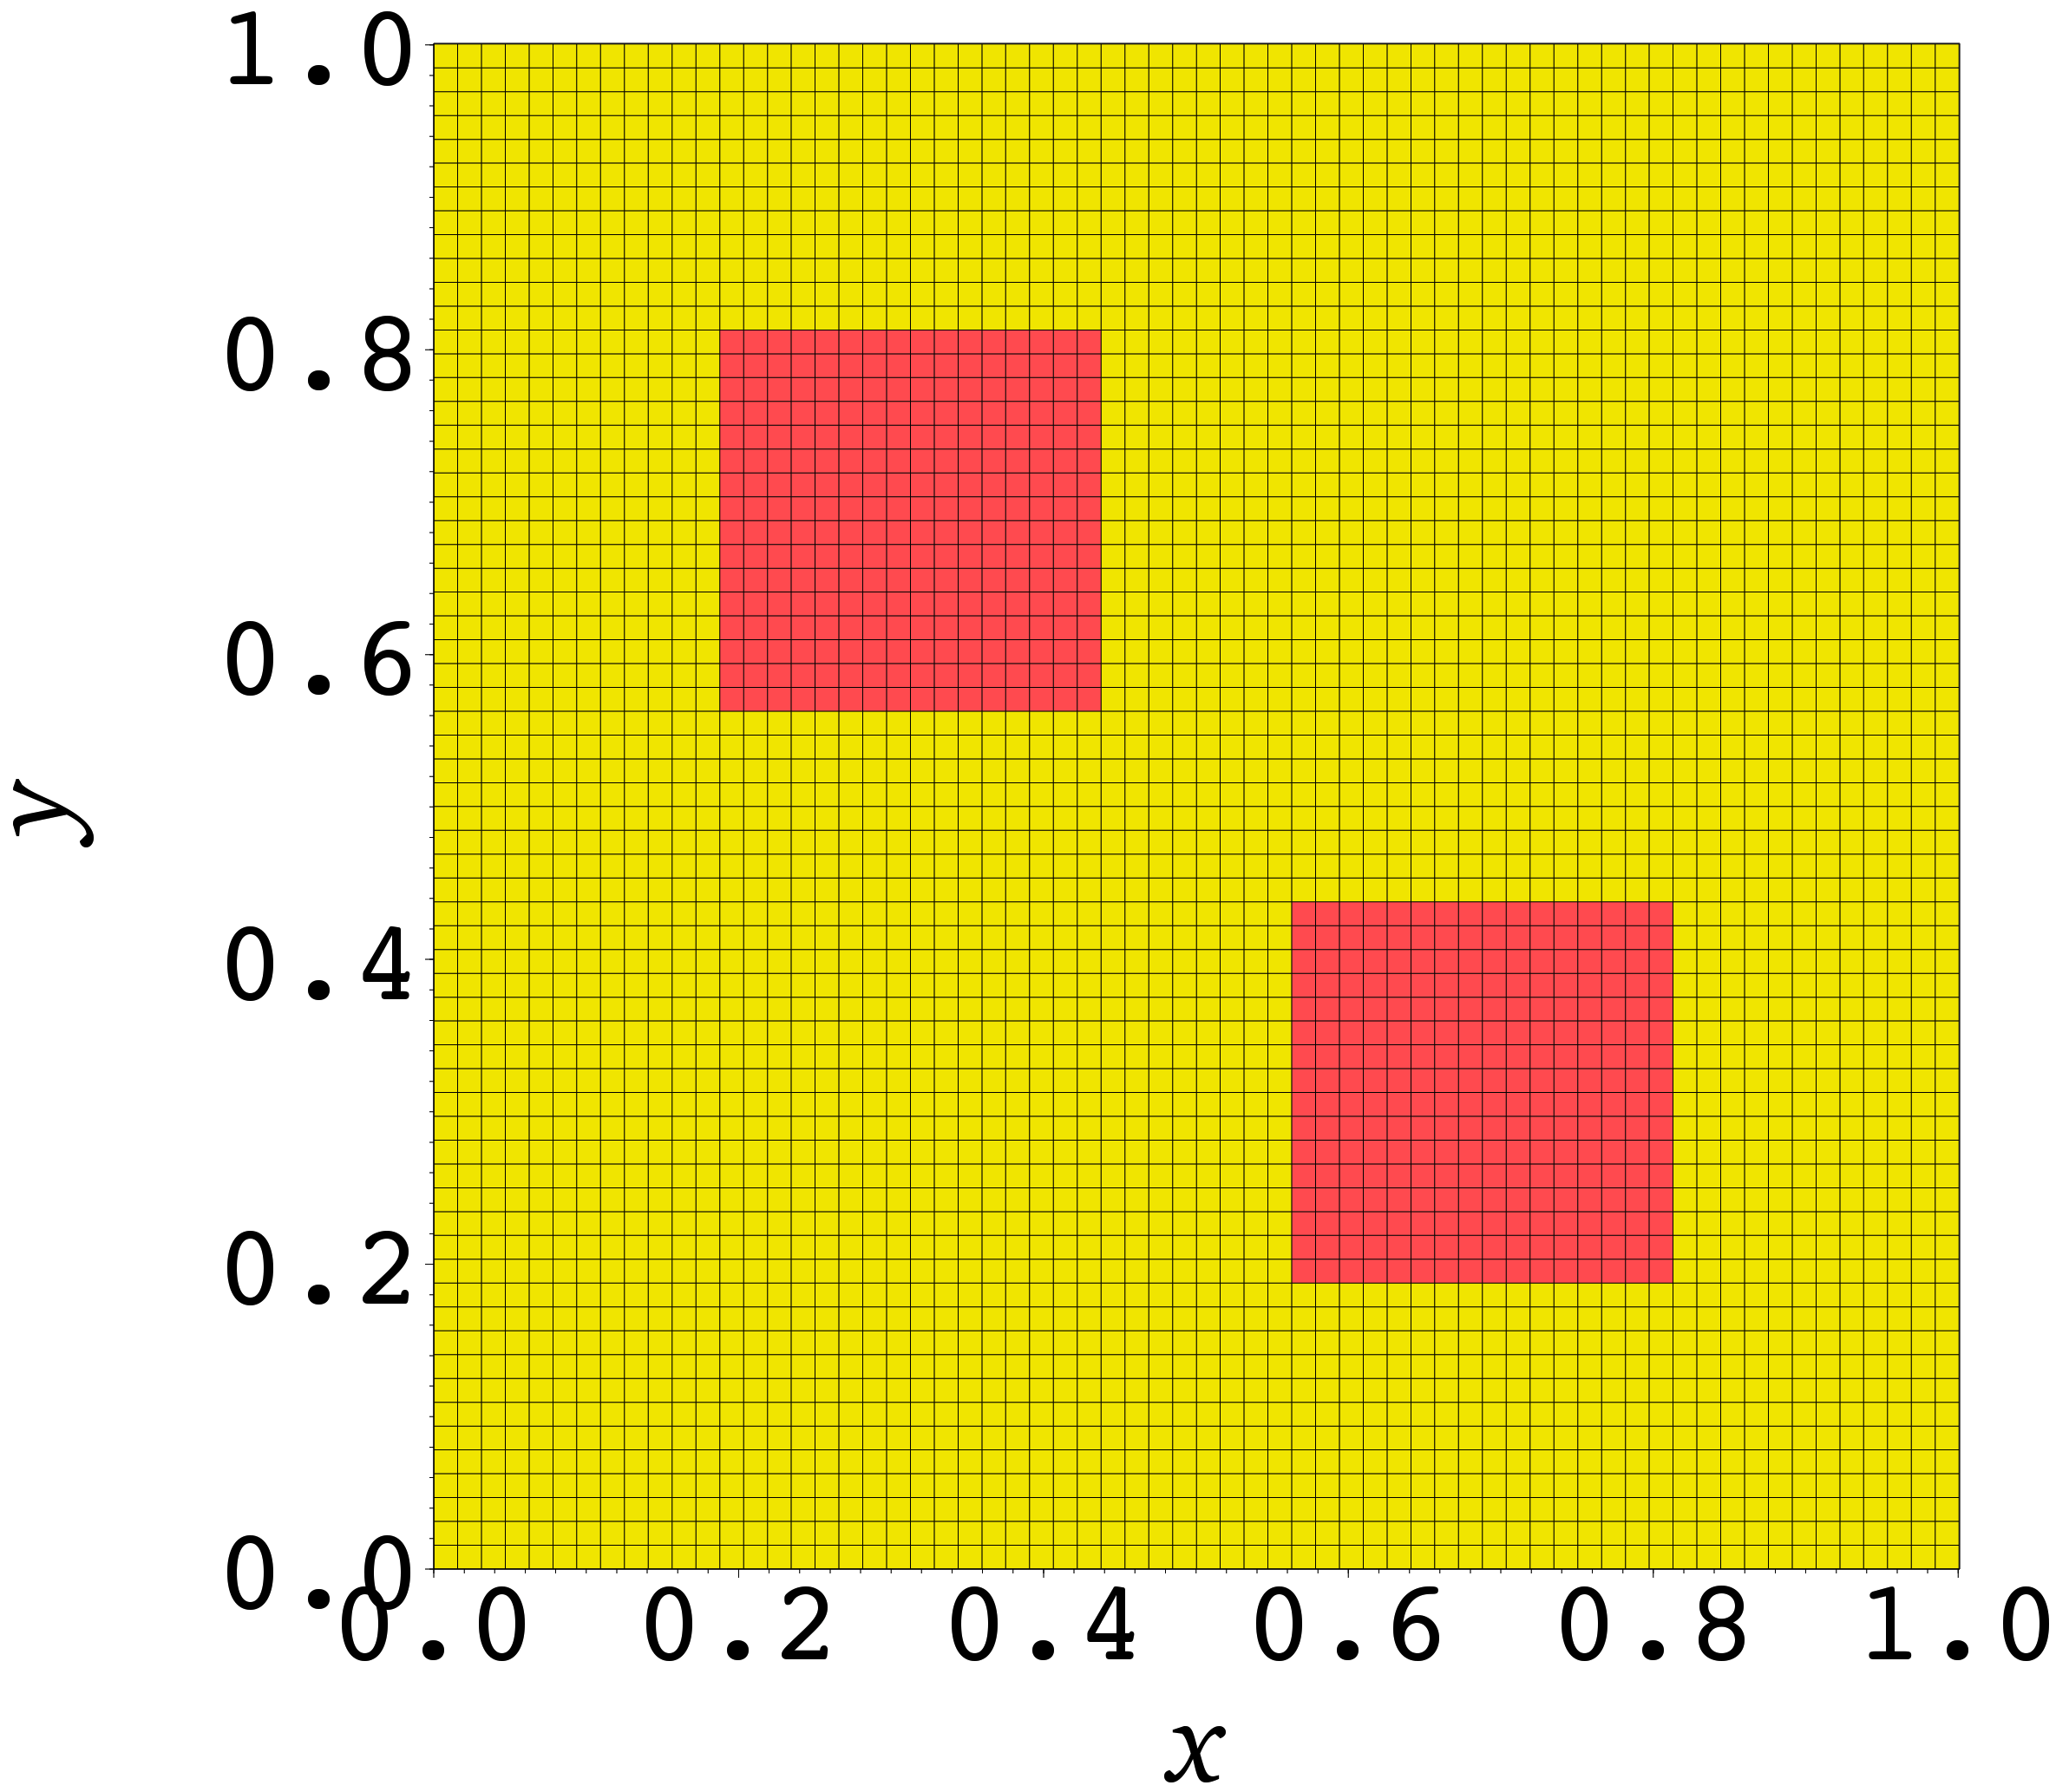
\includegraphics[width=.99\textwidth]{crashpipe-OBSOLETE/materials}
\end{center}
\end{frame}

%%%%%%%%%%%%%%%%%%%%%%%%%%%%%%%%%%%%%%%%
\begin{frame}{Time evolution of material temperature}
\begin{center}
  {\tiny (Replaced with movie)}

  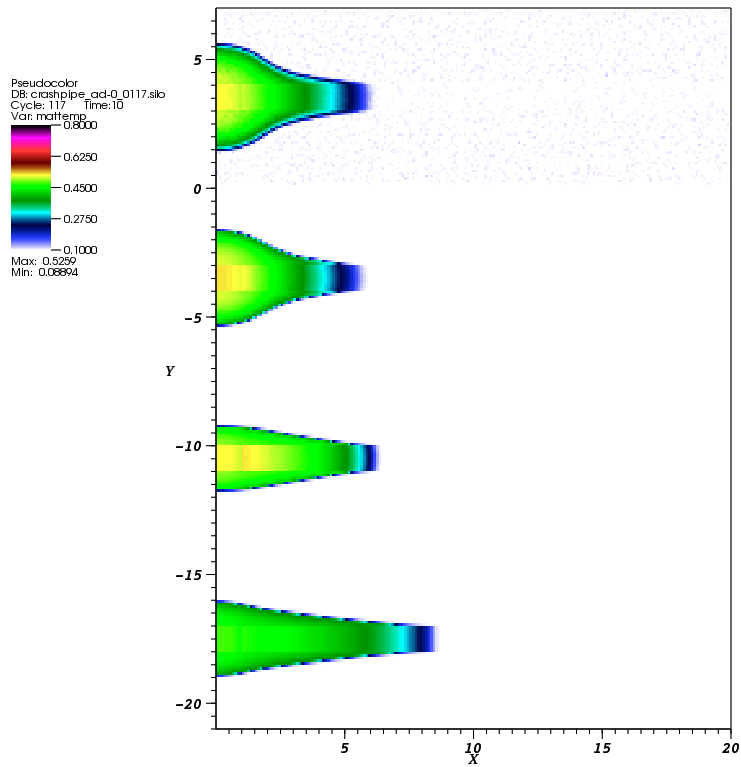
\includegraphics[width=.80\textwidth]{crashpipe-OBSOLETE/mattemp_2d0117}
\end{center}
\end{frame}
%%%%%%%%%%%%%%%%%%%%%%%%%%%%%%%%%%%%%%%%
\begin{frame}{Time evolution of radiation energy density}

\only<1>{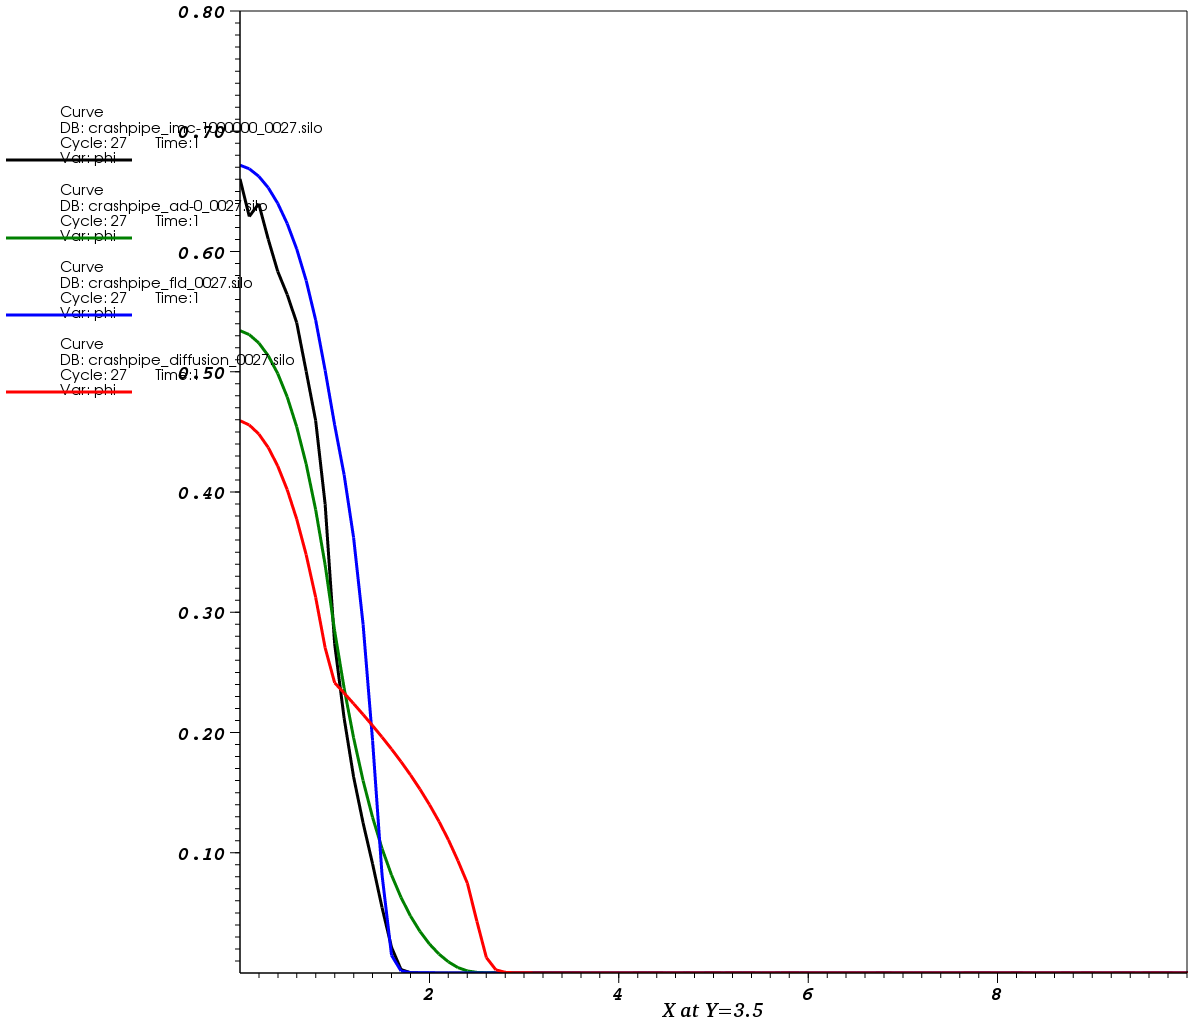
\includegraphics[width=.48\textwidth]{crashpipe-OBSOLETE/phix_t1}}
\only<2>{\includegraphics[width=.48\textwidth]{crashpipe-OBSOLETE/phix_t2}}
\only<3>{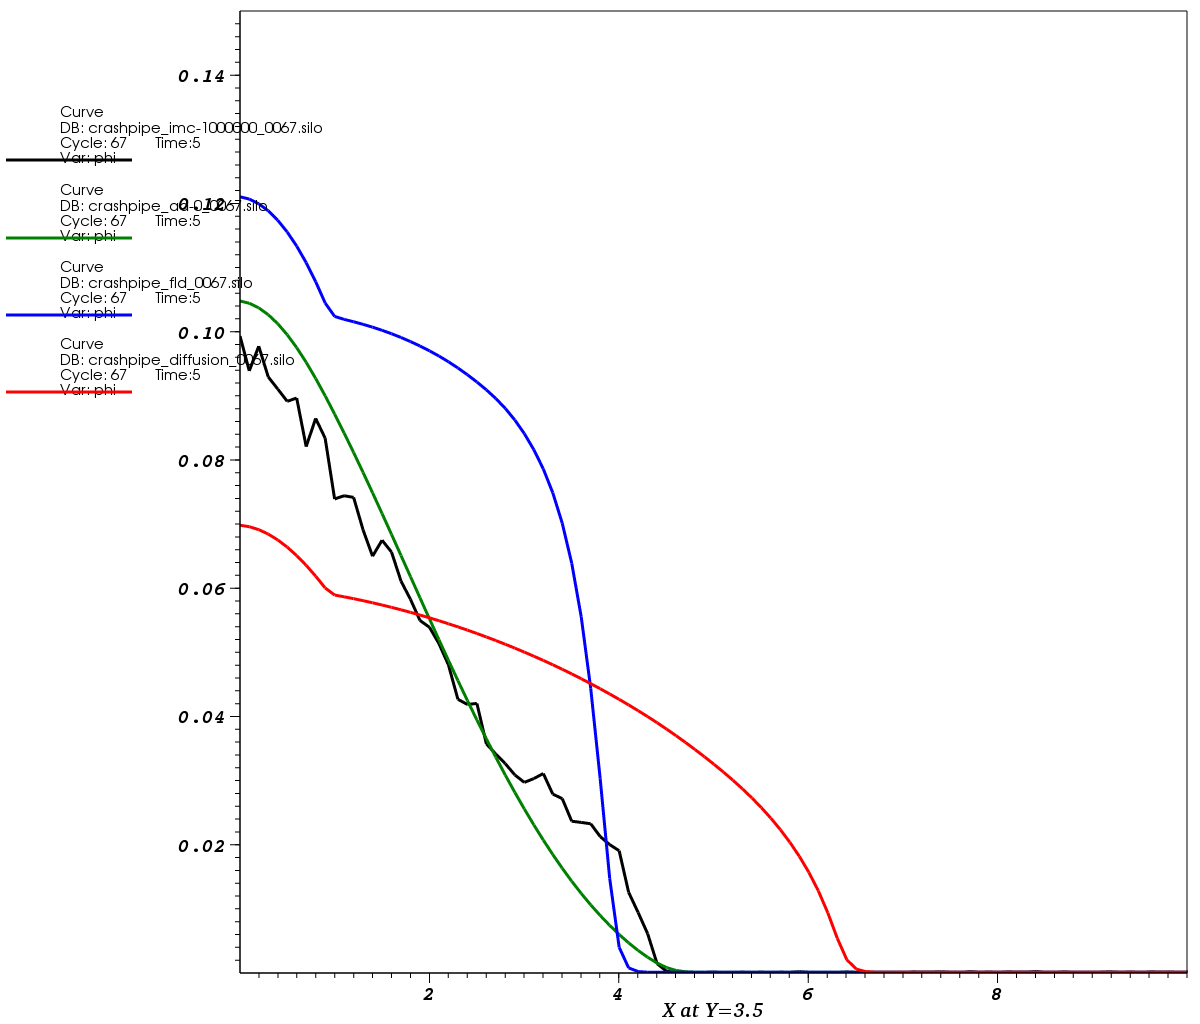
\includegraphics[width=.48\textwidth]{crashpipe-OBSOLETE/phix_t5}}
\only<4>{\includegraphics[width=.48\textwidth]{crashpipe-OBSOLETE/phix_t10}}
\only<1>{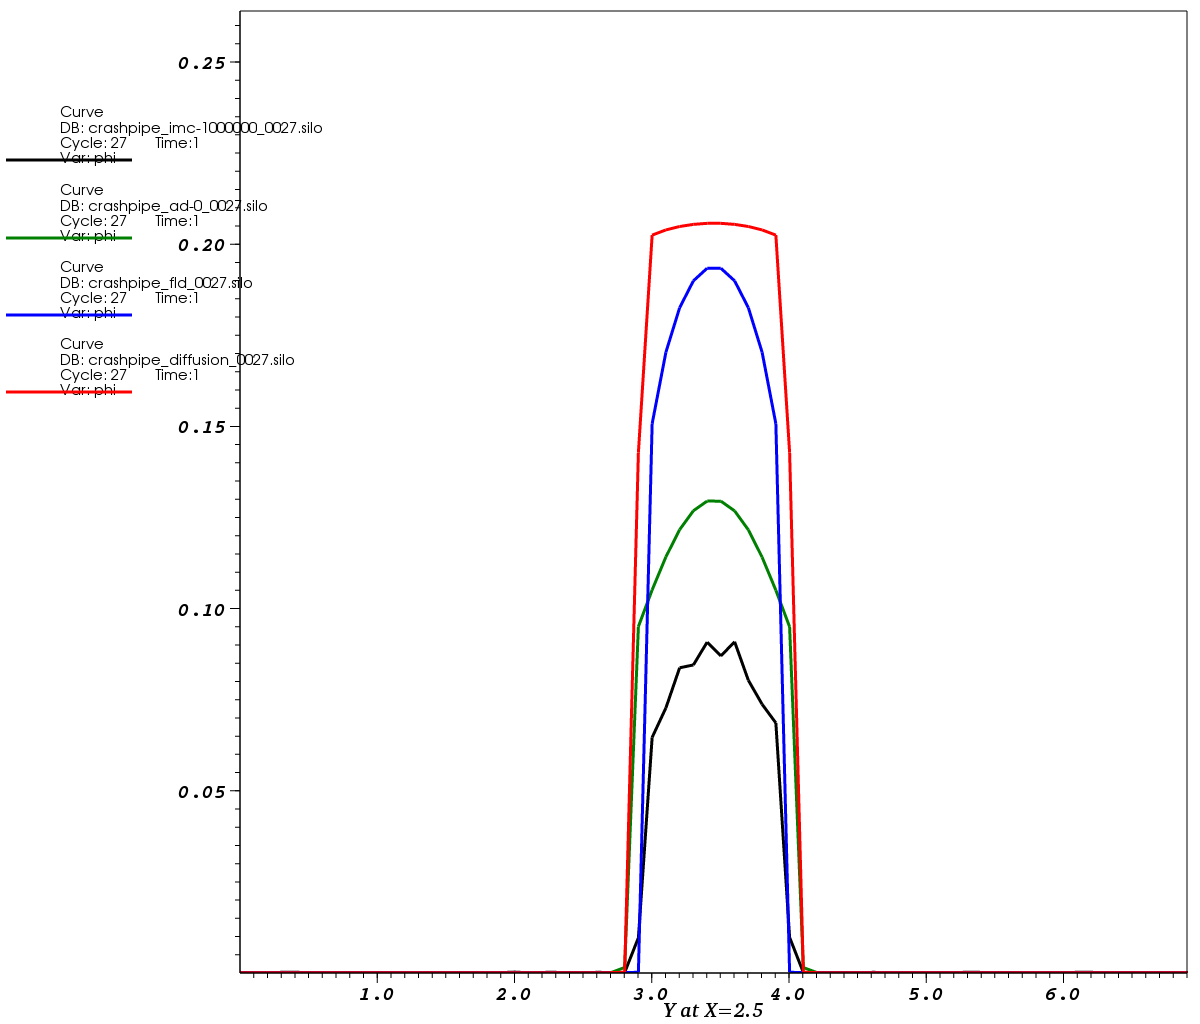
\includegraphics[width=.48\textwidth]{crashpipe-OBSOLETE/phiy_t1}}
\only<2>{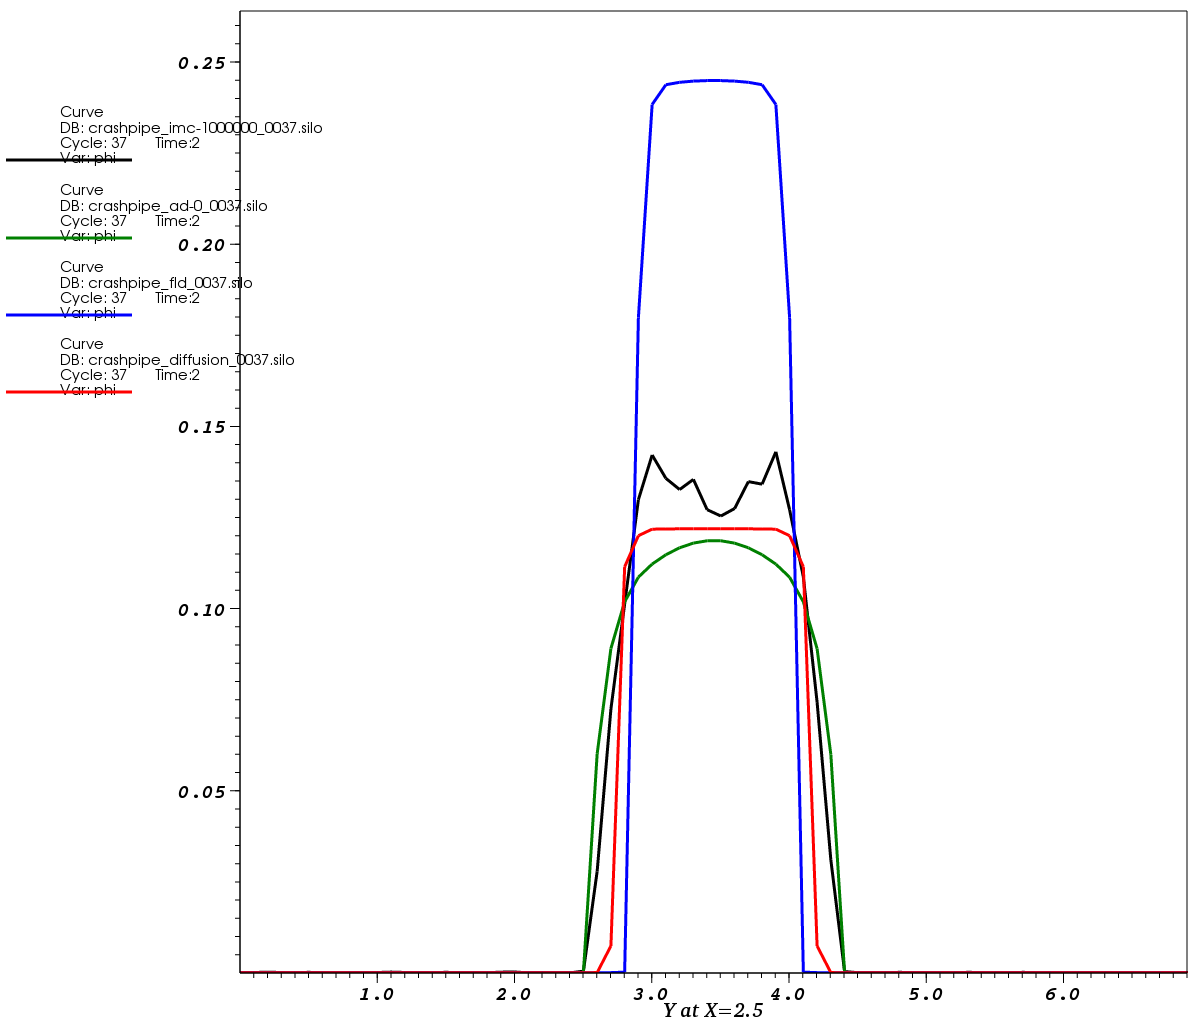
\includegraphics[width=.48\textwidth]{crashpipe-OBSOLETE/phiy_t2}}
\only<3>{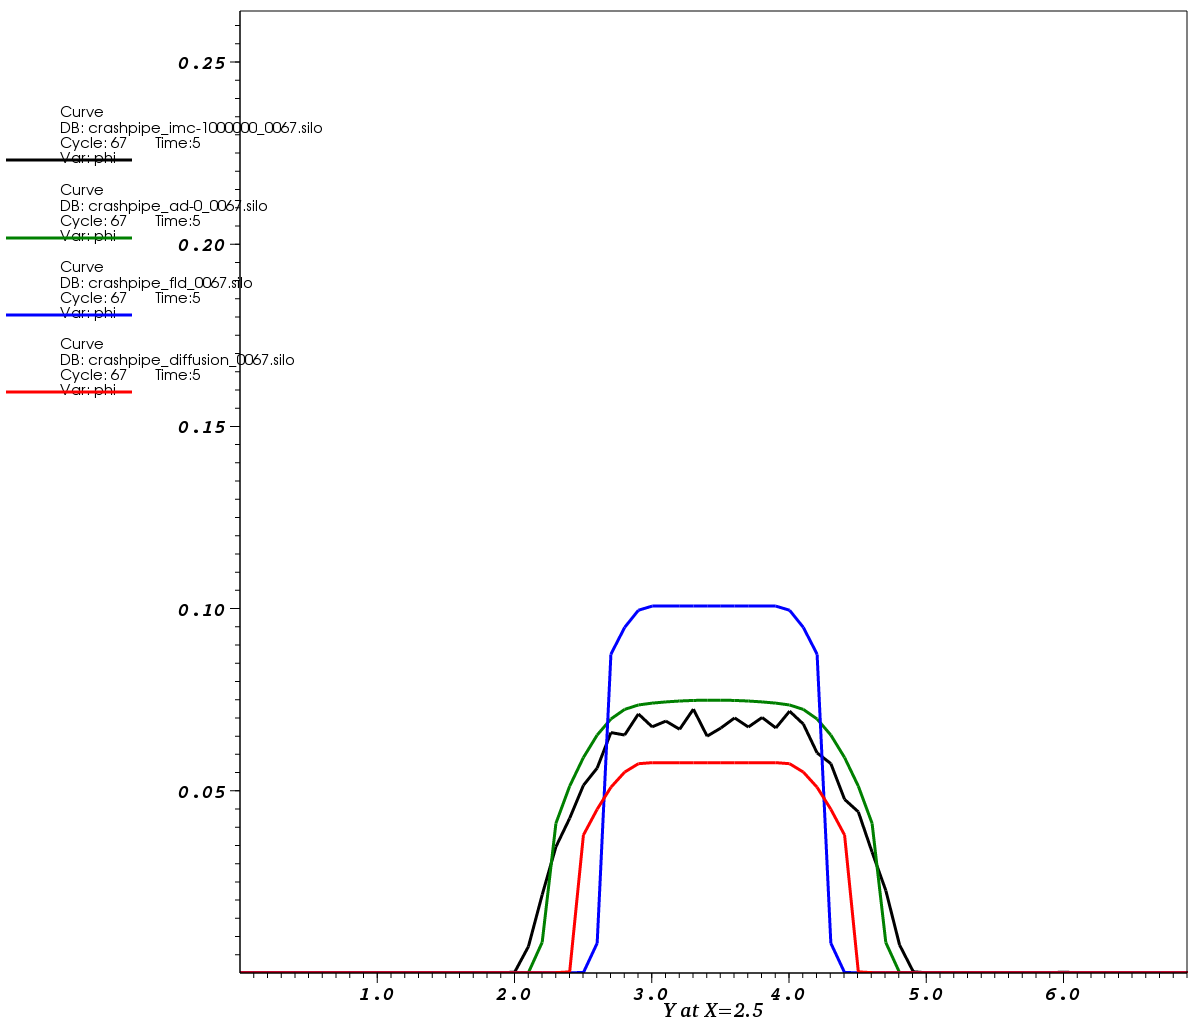
\includegraphics[width=.48\textwidth]{crashpipe-OBSOLETE/phiy_t5}}
\only<4>{\includegraphics[width=.48\textwidth]{crashpipe-OBSOLETE/phiy_t10}}
  
\begin{center}
  along $y=3.5$ \qquad
  \only<1>{ $t=1.0$ }
  \only<2>{ $t=2.0$ }
  \only<3>{ $t=5.0$ }
  \only<4>{ $t=10.0$ }
  \qquad along $x=2.5$

  \textcolor[rgb]{0,0,0}{\textbf{IMC}}\quad
  \textcolor[rgb]{0.1,0.9,0.1}{\textbf{AD}}\quad
  \textcolor[rgb]{0,0,1}{\textbf{FLD}}\quad
  \textcolor[rgb]{1,0,0}{\textbf{Diffusion}}
\end{center}
\end{frame}
%%%%%%%%%%%%%%%%%%%%%%%%%%%%%%%%%%%%%%%%
\begin{frame}{Diffusion coefficients}
\begin{center}
  \includegraphics[width=.60\textwidth]{crashpipe-OBSOLETE/dcoeff_t10}

\textcolor[rgb]{0,0,0}{$D^{xx}$}\quad
\textcolor[rgb]{1,0,.5}{$D^{xy}$}\quad
\textcolor[rgb]{0.1,0.9,0.1}{$D^{yy}$}\quad
\textcolor[rgb]{0,0,1}{$D_\text{FLD}$}\quad
  \textcolor[rgb]{1,0,0}{$D$}
\end{center}
\end{frame}
%%%%%%%%%%%%%%%%%%%%%%%%%%%%%%%%%%%%%%%%
\begin{frame}{Anisotropic diffusion tensor visualization}
\begin{center}
  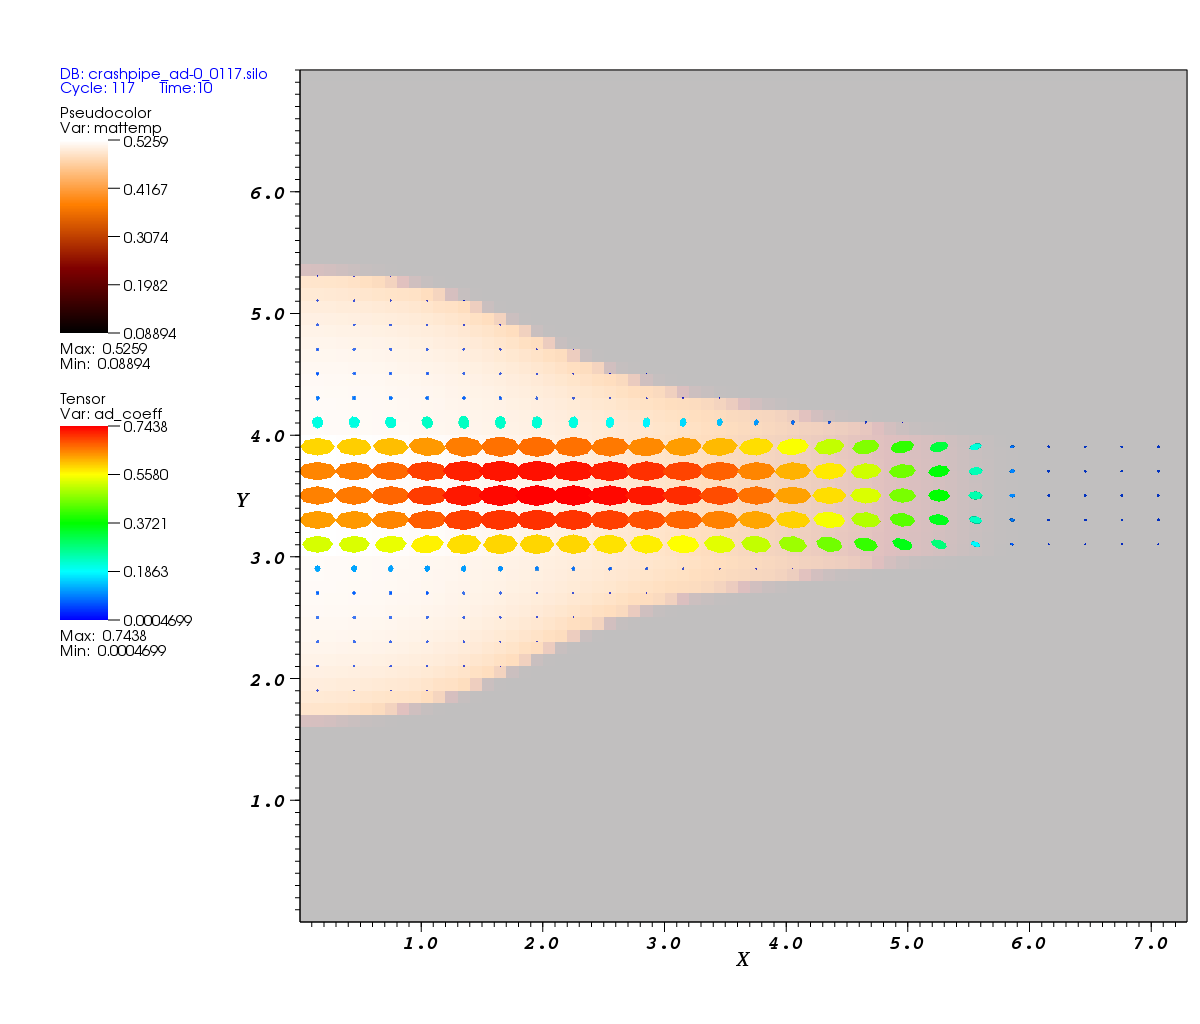
\includegraphics[width=.75\textwidth]{crashpipe-OBSOLETE/adcoeff_t10}
\end{center}
\end{frame}
%%%%%%%%%%%%%%%%%%%%%%%%%%%%%%%%%%%%%%%%
\begin{frame}{Timing results}
  \begin{table}[htb]
    \centering
    \begin{tabular}{cr}
      Method & Time (s) \\ \hline
      IMC & 477 \\
      FLD & 8 \\
      D   & 8 \\
      AD$_{64}$ & 13 \\
      AD$_{128}$ & 22
    \end{tabular}
    \caption{Run times for pipe test problem, 14000 cells. Average of three
    runs.}
    \label{tab:pipeTiming}
  \end{table}
\end{frame}
%%%%%%%%%%%%%%%%%%%%%%%%%%%%%%%%%%%%%%%%%%%%%%%%%%%%%%%%%%%%%%%%%%%%%%%%%%%%
\section{Conclusions}
%%%%%%%%%%%%%%%%%%%%%%%%%%%%%%%%%%%%%%%%
\begin{frame}
  \frametitle{Conclusions}
  Anisotropic diffusion:
  \begin{itemize}
    \item Accounts for some amount of arbitrary anisotropy in angular
      intensity, unlike standard or flux-limited diffusion, by preserving some
      transport physics
    \item Works best in problems with weaker derivatives, as suggested by
      theory and borne out by numerical experiments
    \item Accurately treats the nonlinear time-dependent flow of radiation
      through a tube like that found in CRASH experiments
  \end{itemize}
\end{frame}
%%%%%%%%%%%%%%%%%%%%%%%%%%%%%%%%%%%%%%%%
\begin{frame}
  \frametitle{Future work}
  \begin{itemize}
    \item Improved time-dependent behavior, with wavefront propagation speed of
      $c$
    \item Boundary conditions for both anisotropic diffusion problem and
      purely absorbing transport problem (solution of $f$)
    \item Improve performance by reducing time spent in transport sweeps
      \begin{itemize}
        \item Evaluate $\Dtens$ on coarser spatial grid, since it is smooth
        \item Update $\Dtens$ less frequently
        \item Advanced quadrature set for \emph{a priori} problem geometry
      \end{itemize}
    \item Quantify the penalty of omitting the $D^{xy}$ terms for various
      problems, or find an effective discretization scheme to include them
  \end{itemize}
\end{frame}
%%%%%%%%%%%%%%%%%%%%%%%%%%%%%%%%%%%%%%%%%%%%%%%%%%%%%%%%%%%%%%%%%%%%%%%%%%%%
\appendix
%%%%%%%%%%%%%%%%%%%%%%%%%%%%%%%%%%%%%%%%
\begin{frame}
  \frametitle{Acknowledgments}
  \begin{itemize}
    \item Prof.~Larsen
    \item Committee: Profs.~Martin, Downar, Holloway, Thornton
    \item Funding: NSF, NEUP
  \end{itemize}
\end{frame}

%%%%%%%%%%%%%%%%%%%%%%%%%%%%%%%%%%%%%%%%
\begin{frame}
  \frametitle{Questions?}
\begin{center}
  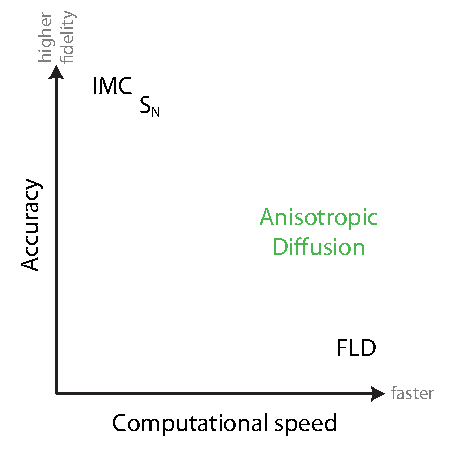
\includegraphics[width=3in]{fidelity2}
\end{center}
\end{frame}

%%%%%%%%%%%%%%%%%%%%%%%%%%%%%%%%%%%%%%%%
\begin{frame}
  \frametitle{References}
\bibliographystyle{ans}
\bibliography{../../SRJall}
\end{frame}
%%%%%%%%%%%%%%%%%%%%%%%%%%%%%%%%%%%%%%%%%%%%%%%%%%%%%%%%%%%%%%%%%%%%%%%%%%%

%	This material is based upon work supported under a National Science
%	Foundation Graduate Research Fellowship. Any opinions, findings, conclusions
%	or recommendations expressed in this publication are those of the author(s)
%	and do not necessarily reflect the views of the National Science
%	Foundation.  
\end{document}
